\problem{Hounded by Indecision}

%\begin{wrapfigure}{r}{0.45\linewidth}
%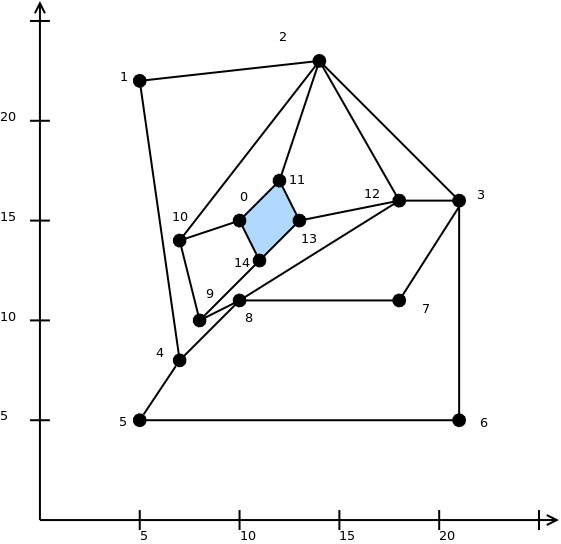
\includegraphics[width=\linewidth]{Gardener/plots1}
%\end{wrapfigure}

OK, maybe stealing the Duchess's favorite ruby necklace was not such a
good idea. You were making your way toward the city gates when you
heard the sound you had been dreading: a sharp whistle followed by an
answering bark. You know that the constable has just fetched his
favorite hound and is starting to search for you.  They might head
straight for a gate. They might try to pick up your trail on the
way. You really can't guess. But if they reach the gate before you,
you're caught. If they happen across your trail, the hound will pick
up your scent. The dog knows your scent already - this isn't your
first offense!  The constable will loose the hound, who can
run \textit{fast} once he has the trail to follow.

You have a dilemma. If you are absolutely sure that you can
reach the gates before the guard and before being overtaken by the
hound, you can keep the necklace. But if you aren't sure, you need to drop
the necklace right now into the nearest pile of rubbish and saunter
casually away. Even if they grab you, without the necklace in your
hands they will eventually release you.

So, keep the necklace or drop the necklace?

\hrulefill

The town is modeled as a rectangular maze of discrete squares.  It is
surrounded by a wall that contains one or more exits. You know, of
course, your own position within the town. You also know the location
of the kennel where the constable and the hound start out.

\begin{itemize}

\item In each turn (unit of time), you, the constable, and the hound 
move simultaneously. 

\item You can move zero or one square(s) horizontally or vertically per turn.

\item Initially, the constable and hound move together, also zero or 
one square(s) vertically or horizontally.

\item If the constable and the hound, moving together, reach a square
that you have previously occupied, the hound catches your scent and
the constable looses the hound. On each subsequent turn, the hound
follows your trail at a speed of one or two squares per turn. (The hound
moves two squares unless doing so would cause it to jump over the
thief or the exit.)

\item If the constable and/or the hound overtake you  (occupy the same
square as you), you are caught. To escape, you must reach an exit at
least one turn before the constable and/or hound.

\end{itemize}

\subsection*{Input}

Input consists of one or more mazes. Each maze begins with a line
containing two integers, $W$ and $H$, $3 \leq W,H \leq 40$, 
denoting the width and the height of
the maze. End of input is indicated when either of these values is
less than $3$.

This is followed by $H$ lines of input, each containing $W$
characters. 

The interpretation of the characters in these lines is as follows:

\begin{itemize}
\item ` ' denotes an open space

\item `K' is an open space denoting the kennel and hence the starting
position of the constable and the hound.  There will be exactly one of
these in any maze.

\item `T' is an open space denoting the original position of the thief
(you).  There will be exactly one of these in any maze.

\item `X' denotes a wall.

\item `E' is an open space representing an exit (a city gate). There will be at
least one of these. 

    All exits will occur on the outer perimeter (as defined by the W
    and H values) of the maze.

\end{itemize}


All mazes will be completely enclosed by a combination of `X' and `E'
characters.  There will be a path from the thief's starting location
to each exit and from the kennel to each exit.

\subsection*{Output}

For each maze, print a single line of output. If there is a path that
you can take that will guarantee that you can escape no matter what path
the constable and hound take, then print ``KEEP IT''.  If there is
no path that offers such a guarantee, print ``DROP IT''.






\subsection*{Example}

Given the input:

\clearpage
\verbfile{Hounded/test0.in}


the output should be:

\verbfile{Hounded/test0.expected}

In both cases, we can pretty much ignore the exit at the bottom of the
maze. The constable can always get there before the thief.

In the first case, if the thief heads straight for the exit on the
left, he emerges from the ``door'' on turn 4, and reaches the exit on
turn 11. On turn 7, the constable can reach the space where the thief
had been on turn 4, and would then loose the hound, which also reaches
the exit on turn 11, catching the thief.

In the second case, the thief has the option of taking the ``side
door'' out of the house, then heading for the wall before turning
right and heading for the exit. It's actually a longer path, taking 13
turns to reach the exit. But the constable won't reach the exit before
turn 14, and the earliest that the constable could
pick up the thief's trail would be on turn 11 (at the thief's staring
location), at which point the constable and hound are too far away to
catch the thief.
